%%%%%%%%%%%%%%%%%%%%%%%%%%%%%%%%%%%%%%%%%
% baposter Landscape Poster
% LaTeX Template
% Version 1.0 (11/06/13)
%
% baposter Class Created by:
% Brian Amberg (baposter@brian-amberg.de)
%
% This template has been downloaded from:
% http://www.LaTeXTemplates.com
%
% License:
% CC BY-NC-SA 3.0 (http://creativecommons.org/licenses/by-nc-sa/3.0/)
%
%%%%%%%%%%%%%%%%%%%%%%%%%%%%%%%%%%%%%%%%%

%----------------------------------------------------------------------------------------
%	PACKAGES AND OTHER DOCUMENT CONFIGURATIONS
%----------------------------------------------------------------------------------------

\documentclass[a0paper,portrait,fontscale=0.2975]{TUTposter} % Adjust the font scale/size here

\usepackage[numbers]{natbib}         % citation style AUTHOR (YEAR), or AUTHOR [NUMBER]
%\setcitestyle{round} % round brackets for citep and citet

\usepackage{graphicx} % Required for including images
\graphicspath{{../img/}} % Directory in which figures are stored

\usepackage{amsmath} % For typesetting math
\usepackage{amssymb} % Adds new symbols to be used in math mode
\usepackage{multirow}

\usepackage{booktabs} % Top and bottom rules for tables
\usepackage{enumitem} % Used to reduce itemize/enumerate spacing
\usepackage{palatino} % Use the Palatino font
%\usepackage{charter}
\usepackage[font=small,labelfont=bf, labelformat=empty]{caption} % Required for specifying captions to tables and figures

\usepackage{url}
\usepackage[capbesideposition=outside,capbesidesep=quad]{floatrow}

\usepackage{multicol} % Required for multiple columns
\setlength{\columnsep}{2em} % Slightly increase the space between columns
\setlength{\columnseprule}{0mm} % No horizontal rule between columns

\setlist[itemize]{itemsep=2pt, topsep=3pt, parsep=0pt,leftmargin=2em}
\setlist[description]{itemsep=2pt, topsep=3pt, parsep=0pt, font=\normalfont\emph, leftmargin=5ex}
\setlist[enumerate]{itemsep=2pt, topsep=3pt, parsep=0pt}
%\newcommand{\compresslist}{ % Define a command to reduce spacing within itemize/enumerate environments, this is used right after \begin{itemize} or \begin{enumerate}
%\setlength{\itemsep}{1pt}
%\setlength{\parskip}{0pt}
%\setlength{\parsep}{0pt}
%}

\usepackage{fix-cm} 
\usepackage{xcolor}   

\makeatletter
\newcommand\HUGE{\@setfontsize\Huge{35}{45}}
\makeatother   

\definecolor{bgr}{RGB}{229, 229, 229} % Defines the color used for content box headers

\title{Planning for Transportation Problems} % Poster title

\author{Ondrej \v{S}kopek} % Author(s)

\newcommand{\insertdepartment}{Department of Theoretical Computer Science and Mathematical Logic}
\newcommand{\institute}{Faculty of Mathematics and Physics, Charles University} % Institution(s)
\newcommand{\comment}[1]{}

\begin{document}

\begin{poster}
{
headerborder=open, % Adds a border around the header of content boxes
colspacing=2.25em, % Column spacing
bgColorOne=bgr, % Background color for the gradient on the left side of the poster
bgColorTwo=bgr, % Background color for the gradient on the right side of the poster
borderColor=white, % Border color
headerColorOne=white, % Background color for the header in the content boxes (left side)
headerColorTwo=white, % Background color for the header in the content boxes (right side)
headerFontColor=black, % Text color for the header text in the content boxes
boxColorOne=white, % Background color of the content boxes
textborder=rectangle, % Format of the border around content boxes, can be: none, bars, coils, triangles, rectangle, rounded, roundedsmall, roundedright or faded
eyecatcher=false, % Set to false for ignoring the left logo in the title and move the title left
headerheight=0.1\textheight, % Height of the header
boxshade=plain,
headershape=rectangle, % Specify the rounded corner in the content box headers, can be: rectangle, small-rounded, roundedright, roundedleft or rounded
headerfont=\hspace{0.2em}\LARGE\bf\textsc, % Large, bold and sans serif font in the headers of content boxes
%textfont={\setlength{\parindent}{1.5em}}, % Uncomment for paragraph indentation
linewidth=0pt, % Width of the border lines around content boxes
boxpadding=1.2em,
boxheaderheight=3em
}
%----------------------------------------------------------------------------------------
%	TITLE SECTION 
%----------------------------------------------------------------------------------------
%
{\includegraphics[height=30em]{logo-en.pdf}} % First university/lab logo on the left
{\vspace{0.8em}\hspace{0.5em}\HUGE\textsf{\textcolor{black}{Planning for Transportation Problems}}\vspace{0.3em}%
} % Poster title
{%
\LARGE\textsf{Ondrej {\v{S}}kopek}\\%
}
%{\includegraphics[width=36em]{logo-en.pdf}} % Second university/lab logo on the right

%----------------------------------------------------------------------------------------
%	OBJECTIVES
%----------------------------------------------------------------------------------------

\headerbox{Introduction}{name=introduction,column=0,row=0,span=1}{

\vspace{-1em}
\begin{flushleft}
Our goal is to design \textit{domain-specific} planners 
for several variants of the \textit{Transport} domain, used in International Planning Competitions (IPC).

\vspace{0.3em}

\textbf{Transport domain}:
\vspace{-0.3em}
\begin{itemize}
\item road network with items located at specified locations
\item items are to be delivered to their destinations
\item using a fleet of (different) vehicles
\item \textit{Goal}: deliver all items
with the least total cost or duration
\end{itemize}
\end{flushleft}
}




%----------------------------------------------------------------------------------------
%	REFERENCES
%----------------------------------------------------------------------------------------

\headerbox{References}{name=references,column=0,above=bottom,span=1}{

\vspace{-0.5em}
\begin{flushleft}
\renewcommand{\section}[2]{\vskip 0.05em} % Get rid of the default "References" section title
\nocite{*} % Insert publications even if they are not cited in the poster
\scriptsize{ % Reduce the font size in this block
\vspace{-0.9em}
\setlength{\bibsep}{0pt plus 0.3ex}
\bibliographystyle{plain}
\bibliography{../../bp/en/bibliography-poster.bib} % Use sample.bib as the bibliography file
\vspace{-0.8em}
}
\end{flushleft}
}

%----------------------------------------------------------------------------------------
%	MATERIALS AND METHODS
%----------------------------------------------------------------------------------------

\headerbox{Materials \& Methods}{name=method,column=0,below=introduction}{ % This block's bottom aligns with the bottom of the conclusion block

\vspace{-1em}
\begin{flushleft}
Our planners are compared to those taking part in past IPCs. Experiments were run using:
\vspace{-0.1em}
\begin{itemize}
\item 30 minutes of CPU time
\item 4 GB of RAM
\item limited to one core per planner
\item run on the clusters of MetaCentrum
\end{itemize}

\vspace{0.1em}
\textbf{Sequential planners}:
\vspace{0.1em}

{
\setlength{\tabcolsep}{3pt} % General space between cols (6pt standard)
\renewcommand{\arraystretch}{1} % General space between rows (1 standard)
\begin{tabular}{@{}ll}
\multirow{2}{*}{\textit{MSFA3}} & Meta-heuristically weighted SFA\\
&  with package and vehicle distance\\[4pt]
\multirow{2}{*}{\textit{MSFA5}} & Meta-heuristically weighted SFA\\
& with the general marking heuristic\\[4pt]
\textit{RRAPN} & Rand. Restart Around Path Nearby
\end{tabular}

\vspace{0.4em}
\textbf{Temporal planners}:
\vspace{0.1em}

{
\setlength{\tabcolsep}{2pt} % General space between cols (6pt standard)
\renewcommand{\arraystretch}{1} % General space between rows (1 standard)
\begin{tabular}{@{}ll}
\textit{MSFA5Sched} & Scheduled MSFA5\\[2pt]
\textit{RRAPNSched} & Scheduled RRAPN\\[2pt]
\textit{TRRAPN} & Temporal RRAPN
\end{tabular}
}
}
\end{flushleft}
}






%----------------------------------------------------------------------------------------
%	RESULTS
%----------------------------------------------------------------------------------------

\headerbox{Results}{name=results,column=1,row=0,span=2}{

\vspace{-1.3em}
\begin{multicols}{2}
\begin{flushleft}
We have designed Transport planners that are able to beat
all planners from the:
\begin{itemize}
\item sequential and temporal tracks of IPC 2008 (Figure~1 and 2)
\item sequential track of IPC 2011 (Figure~3)
\end{itemize}

\vspace{0.5em}
In the 2014 IPC (Figure 4), we would have attained second place, behind the impressive result of Mercury (domain-independent).

\vspace{0.5em}
Our planners perform well across datasets, as can be observed in Table~1 and 2.

\vspace{0.7em}
\footnotesize{Figures only show the three best planners from IPC on
each dataset.}

\begin{center}
\small
\begin{tabular}{lr}
\toprule
\textbf{Planner} & \textbf{Avg.\;quality}\\
\midrule
MSFA3 & 0.923\\
MSFA5 & \textbf{0.924}\\
RRAPN & 0.894\\
\bottomrule
\end{tabular}
\vspace{-0.5em}
\captionof{table}{\textbf{Table 1:} Average quality on sequential datasets.}

\vspace{1em}
\begin{tabular}{lr}
\toprule
\textbf{Planner} & \textbf{Avg.\;quality}\\
\midrule
MSFA5Sched & 0.483\\
RRAPNSched & 0.905\\
TRRAPN & \textbf{0.934}\\
\bottomrule
\end{tabular}
\vspace{-0.5em}
\captionof{table}{\textbf{Table 2:} Average quality on the temporal dataset.}
\end{center}
\end{flushleft}
\end{multicols}

\vspace{-1.5em}
\begin{center}
\floatbox[{\capbeside\thisfloatsetup{capbesideposition={right,center},
capbesidewidth=9em}}]{figure}[0.4\paperwidth]
{\caption{\textbf{Figure 1:} IPC 2008\\Sequential satisficing}}
{\includegraphics[width=0.92\linewidth]{seq-sat-6-quality.pdf}}

\vspace{0.4em}
\floatbox[{\capbeside\thisfloatsetup{capbesideposition={right,center},
capbesidewidth=9em}}]{figure}[0.4\paperwidth]
{\caption{\textbf{Figure 2:} IPC 2008\\Temporal satisficing}}
{\includegraphics[width=0.92\linewidth]{tempo-sat-6-quality.pdf}}

\vspace{0.4em}
\floatbox[{\capbeside\thisfloatsetup{capbesideposition={right,center},
capbesidewidth=9em}}]{figure}[0.4\paperwidth]
{\caption{\textbf{Figure 3:} IPC 2011\\Sequential satisficing}}
{\includegraphics[width=0.92\linewidth{}]{seq-sat-7-quality.pdf}}

\vspace{0.4em}
\floatbox[{\capbeside\thisfloatsetup{capbesideposition={right,center},
capbesidewidth=9em}}]{figure}[0.4\paperwidth]
{\caption{\textbf{Figure 4:} IPC 2014\\Sequential satisficing}}
{\includegraphics[width=0.92\linewidth{}]{seq-sat-8-quality.pdf}}
\end{center}
\vspace{-2.4em}
}







%----------------------------------------------------------------------------------------
%	Acknowledgements
%----------------------------------------------------------------------------------------

\headerbox{Acknowledgements}{name=ack,column=1,span=1,aligned=references}{

\vspace{-1em}
\begin{flushleft}
\footnotesize
Thank you to prof.\,RNDr.\,Roman\,Bart{\'{a}}k,\,Ph.D.,\\
my advisor.
\vspace{0.8em}

Provided access to the computing facilities of
MetaCentrum is greatly appreciated.

\vspace{-0.22em}
\phantom{a}
\end{flushleft}
}

%----------------------------------------------------------------------------------------
%	TE
%----------------------------------------------------------------------------------------

\headerbox{TransportEditor}{name=te,column=0,span=1,below=method,above=references}{

\vspace{-1.5em}
\begin{flushleft}
Editor for transportation problem analysis and planner design \citep{Skopek2017}.
\begin{center}
\vspace{-0.5em}
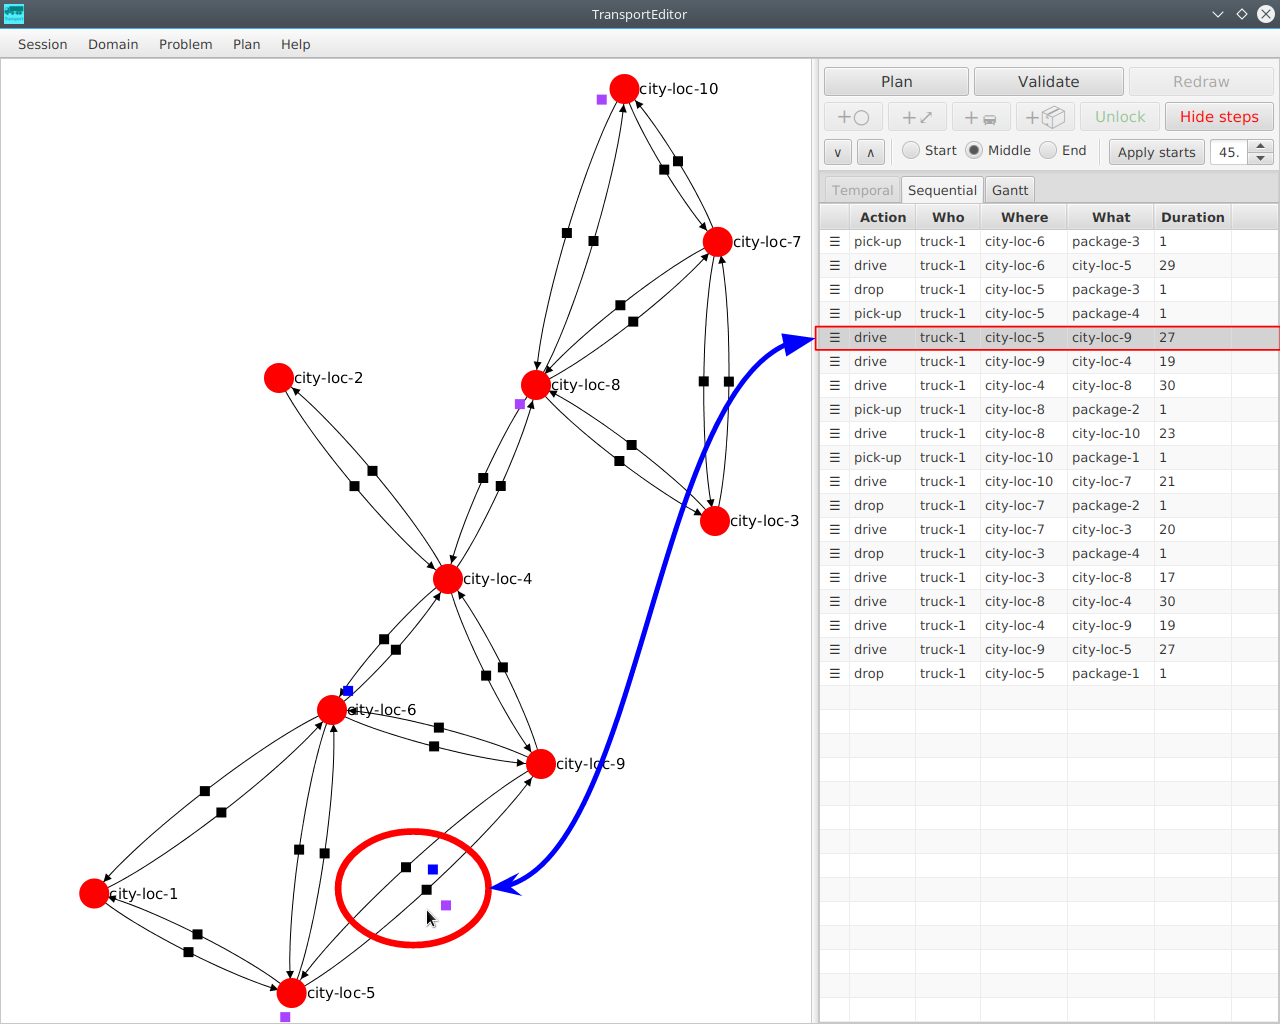
\includegraphics[width=\linewidth{},height=14em]{../../bp/img/transporteditor_planstates.png}
\captionof{figure}{\textbf{Figure 5:} Tracing a plan in TransportEditor.}
\end{center} 
Will be presented at the System Demonstrations track of ICAPS 2017.
\end{flushleft}
}

%----------------------------------------------------------------------------------------
%	CONCLUSION
%----------------------------------------------------------------------------------------

\headerbox{Conclusion}{name=conclusion,column=1,span=1,below=results,above=ack}{

\vspace{-1.5em}
\begin{flushleft}
\small
\begin{itemize}[leftmargin=1em,itemsep=0.3em]
\item \textbf{Domain knowledge} can be \textbf{effectively used}
to generate better plans faster.
\item State-of-the-art \textbf{domain-independent planners}
are often very \textbf{effective} even without domain knowledge.
\end{itemize}
\end{flushleft}
}

\headerbox{}{name=logo,column=2,span=1,aligned=ack,
,boxpadding=0em,bottomaligned=ack}{
\vspace{1.2em}
\begin{center}
\includegraphics[trim={1.5em 2em 0em 2.5em},clip, width=29em]{logo-en.pdf}
\end{center}
}

%----------------------------------------------------------------------------------------
%	Further Information
%----------------------------------------------------------------------------------------

\headerbox{Further Information}{name=further,column=2,span=1,aligned=conclusion,bottomaligned=conclusion,boxpadding=0.8em}{

\vspace{-0.8em}
\begin{flushleft}
\setlength{\tabcolsep}{0.4em}
\footnotesize
\begin{tabular}{@{}cl@{}}
\parbox[c]{1.5em}{\includegraphics[width=1.5em]{github.pdf}} & \url{github.com/oskopek/TransportEditor} \\[1em]
\parbox[c]{1.5em}{\includegraphics[width=1.5em]{mail.pdf}} & \url{oskopek@oskopek.com} \\[1em]
\textsc{WWW} & \url{oskopek.com/docs/bc-thesis.pdf}
\end{tabular} 
\end{flushleft}
}

%----------------------------------------------------------------------------------------

\end{poster}

\end{document}
